\section*{Reproducibility Summary}


\subsubsection{Scope of Reproducibility}
In this work, we aim to reproduce the findings of the paper "Optimizing Deep Learning Inference on Embedded Systems Through Adaptive Model Selection"\supercite{marco2019optimizing}. This paper presents/introduces ... premodel ... knn .. CNN .. embedded systems.

\subsubsection{Methodology}
TBD

\subsubsection{Results}
TBD

\subsubsection{What was easy}
TBD

\subsubsection{What was difficult}
TBD

\subsubsection{Communication with original authors}
We did not contact the authors of the original paper.



\section{Introduction}
Deep learning produces models capable of performing a wide range of complex tasks. However, such models tend to consume a lot of computing power, which is often a limiting factor for using them on embedded systems. While less power-intense models exist, they tend to give less accurate results or even completely fail at harder problems.

Marco et. al. \cite{marco2019optimizing} propose an adaptive model selection method to leverage less power-intense models for simple tasks while employing more powerful models to achieve good results even on complex tasks.

Here we attempt to reproduce their work on the two DNN domains described in the paper: image classification and machine translation.

\section{Scope of Reproducibility}
Authors have the following claims:
\begin{itemize}
    \item \textbf{Claim 1: image classification top-1 accuracy improvement.}

          The authors claim that ...

    \item \textbf{Claim 2: image classification reduction in inference time.}

          The authors claim that ...

    \item \textbf{Claim 3: machine translation reduce inference time without affecting accuracy.}

          The authors claim ...

\end{itemize}


\section{Methodology}

Our replication effort focused on the adaptive model selection methodology, particularly for image classification and machine translation tasks. To compensate for the absence of official code from the original study, we referred to an \href{https://github.com/qwerybot/Adaptive_Deep_Learning}{archived GitHub repository}, which was related to a previous study\supercite{taylor2018adaptive} by the same authors. This earlier study concentrated specifically on the image classification aspect.

Our approach involved adapting the available resources and developing custom methodologies where necessary. For image classification, we devised our own feature extraction and premodel techniques, drawing insights from the descriptions in the referenced papers. In the area of machine translation, we tackled the challenges posed by dataset discrepancies and the lack of specific methodological details in the original paper.

The objective was to closely emulate the experimental setup of the original study, making informed adaptations to fill in the gaps where explicit details were not provided.

\subsection{Image classification}

Our efforts in the image classification section were focused on the premodel construction and comparison, as the pretrained image classification neural networks are freely available online, and as such require no reproducibility testing. 
\paragraph{Architecture}
The chosen model selector architectures were 16-depth decision tree, a support vector classifier and a K-nearest-neighbours classifier. These were combined into a 3-layer hierarchy, where each further layer only classified those datapoints that the previous ones did not.
\paragraph{Comparison}
The premodel combinations were compared in inference time, as model construction is a pre-processing step and does not affect real-world performance. Furthermore, they were compared in top-1 accuracy versus a hypothetical ideal model selector.

\subsubsection{Premodel}
In the original paper, the premodel is constructed with three consecutive simple models, to estimate large neural network performance. As per the original authors, we tested all configurations of these three models on different hierarchy levels. Our results, however, do not seem to align with those of the original authors. We observed much larger differences in runtime, combined with significantly smaller differences in prediction accuracies. This is likely due to authors' measuring the entire pipeline duration, as opposed to only benchmarking the premodel.

For comparison, runtime and accuracy as they report it is shown in figure \ref{fig:11a_orig}, while our results are shown in \ref{fig:11a_ours}. Some of these differences could be attributed to the lack of clear information on what features the authors used, and how they were extracted or augmented. 
 
 \begin{figure}
    \centering
    \includegraphics{}
    \caption{TODO COPY OF THEIR fig 11a}
    \label{fig:11a_orig}
\end{figure}
 \begin{figure}
    \centering
    \includegraphics{}
    \caption{TODO our results}
    \label{fig:11a_ours}
\end{figure}

\subsection{Machine translation}

\subsubsection{NMT models} % Idk, we should probably explain this situation first, since pretrained NMT models aren't availabe and the whole thing is quite sketchy

In the original article, the authors describe using 15 Tensorflow-NMT~\cite{luong17} models trained on WMT English-German dataset. Unlike the models used in the image classification part, pretrained models used for the machine translation part are not available online. In the original article, the authors mention number of layers and use of gnmt attention as the main difference between the models, but don't provide any other hyperparameters, therefore we assume they match the standard hyperparameters provided by Tensorflow-NMT.

Based on the original article, the models were trained on \textquote*[{\cite[p. 13]{marco2019optimizing}}]{WMT09-WMT14 English-German newstest dataset}; However, when we tried to train Tensorflow-NMT models on that dataset, we were unable to reproduce the results, or even achieve any meaningful training, as shown in \figurename~\ref{fig:tf-nmt_paper_training}.

\begin{figure}[h]
    \centering
    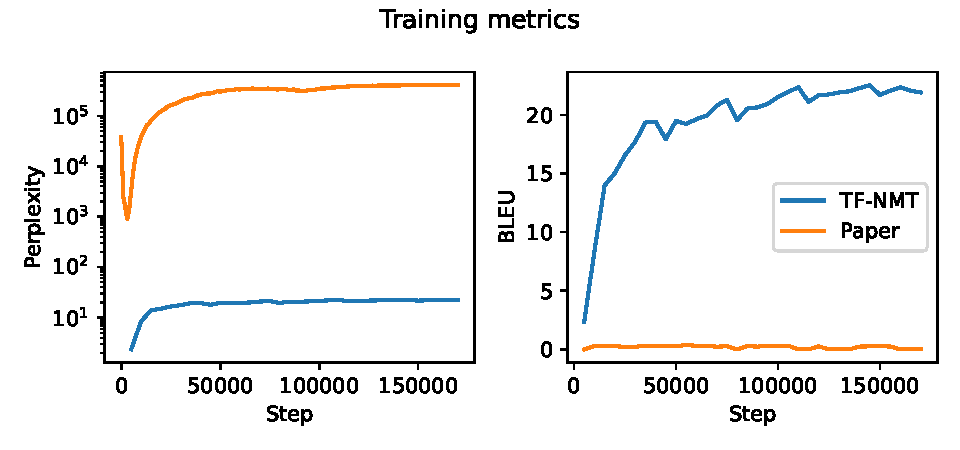
\includegraphics[width=0.75\textwidth]{figures/tf-nmt_paper_training.pdf}
    \caption{Comparison of training metrics when training the same Tensorflow-NMT model on WMT English-German newstest dataset (paper) and the whole WMT English-German dataset used by the Tensorflow-NMT authors (TF-NMT). It's clear that, at least without significant changes to the hyperparameters, the newstest dataset isn't sufficient to train Tensorflow-NMT models.}
    \label{fig:tf-nmt_paper_training}
\end{figure}

Because training the underlying NMT models isn't the primary focus of the original article, we decided to train the models following the standard WMT English-German training described in Tensorflow-NMT and train the four models used in the paper: 3\_layer, gnmt\_2\_layer, gnmt\_4\_layer, and gnmt\_8\_layer. We included hyperparameters and scripts we used to prepare both datasets and train our models with the code. We were unable to determine what the remaining 11 models used by the original authors were, as the original article simply states that they used 15 \textquote*[{\cite[p. 13]{marco2019optimizing}}]{models of varying sizes and architectures} based on Tensorflow-NMT in the model selection step.

% We replicated the model selection algorithm, but without knowing what models the original authors considered in the model selection step, we weren't able to replicate the results for that part.

% ... at this point we got the translations generated by our models along with inference time for each sentence, and we can move to feature engineering and premodel, and try to replicate the main focus points of the original article


\subsection{Feature engineering}
\subsubsection{Image classification}

Our feature engineering efforts for image classification were guided by the features listed in the original study. However, due to the lack of specific details in the original paper, particularly regarding the algorithms used for keypoint detection, edge detection, and hue histogram calculation, we developed our own methods.

\paragraph{Keypoint Detection}
We employed the ORB (Oriented FAST and Rotated BRIEF) algorithm\supercite{Rublee2011ORBAE} for keypoint detection. This choice was based on ORB's efficiency and its ability to detect a large number of keypoints\footnote{\url{https://mikhail-kennerley.medium.com/a-comparison-of-sift-surf-and-orb-on-opencv-59119b9ec3d0}}.

\paragraph{Edge Detection and Analysis}
For edge detection, we used the Canny edge detector\supercite{canny1986computational} combined with contour analysis to calculate edge lengths. This resulted in our edge length histogram bins showing different correlation patterns compared to those reported in the original study. Similarly, for edge angles, we utilized the Sobel operator\supercite{kanopoulos1988design}, which also showed variations in correlation from the original findings.

\paragraph{Hue Histogram}
The calculation of the hue histogram was done using the HSV color space conversion. We noted that our hue histogram bins were less correlated compared to those in the original study.

\paragraph{Aspect Ratio and Area by Perimeter}
For calculating the aspect ratio and area/perimeter ratio of the main object, we used contour detection methods. The specific algorithmic choices were made in the absence of detailed guidance from the original paper.

\paragraph{Correlation Analysis}
Our correlation analysis revealed significant differences from the original study. For instance, the correlation between different hue bins and between various edge angle bins diverged from the patterns reported in the original paper. These differences could potentially impact the effectiveness of the feature set in predictive modeling.

\paragraph{Visualization of Correlations}
To effectively communicate our findings, we have included a heatmap of the Pearson correlation matrix of the features we computed \ref{fig:correlation_matrix}. This visualization provides an intuitive understanding of the relationships between different features in our implementation.

\begin{figure}[h]
    \centering
    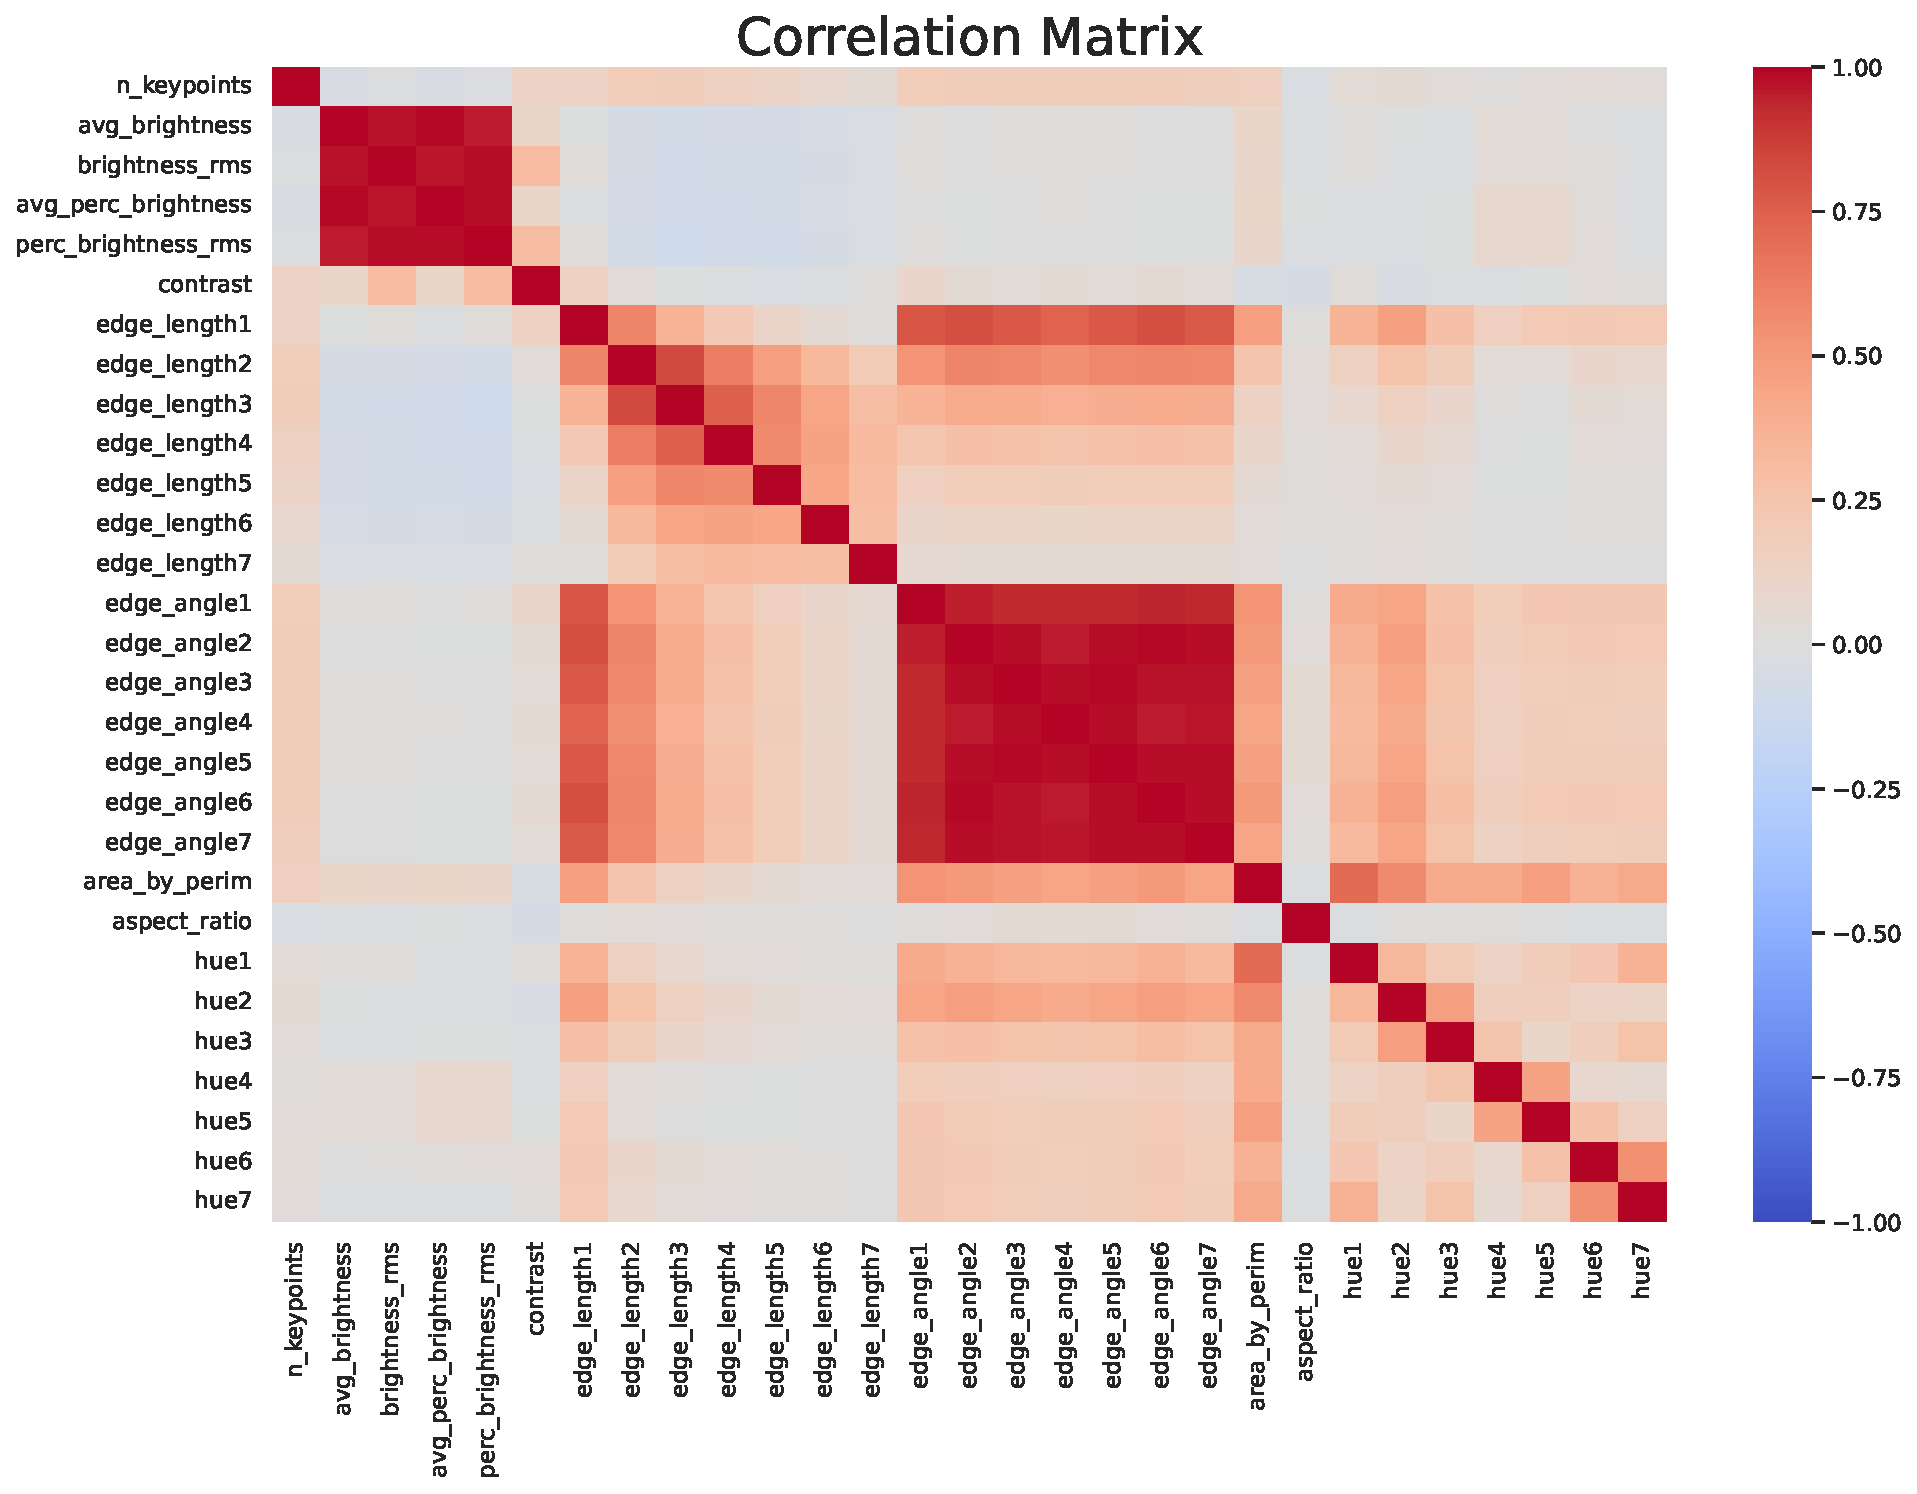
\includegraphics[width=0.75\textwidth]{figures/cv_corr_matrix.pdf}
    \caption{Heatmap of the Pearson correlation matrix for the features in our image classification feature engineering.}
    \label{fig:correlation_matrix}
\end{figure}

It's important to note that these differences in correlations might influence the model's performance and generalizability, and our observations suggest areas where further research and clarification from the original authors might be beneficial.

\begin{table}[h]
    \centering
    \caption{Correlation values (absolute) of removed features to the kept ones for image classification.}
    \begin{tabular}{lll}
        \hline
        \textbf{Kept Feature} & \textbf{Removed Feature} & \textbf{Correl.} \\ \hline
        avg\_brightness       & brightness\_rms          & 0.98             \\
                              & avg\_perc\_brightness    & 0.98             \\
                              & perc\_brightness\_rms    & 0.96             \\
        edge\_angle1          & edge\_angle[2-7]         & 0.92 - 0.95      \\ \hline
    \end{tabular}
\end{table}



\subsubsection{Machine translation}

\paragraph{Feature Selection and Challenges}
In our replication of the machine translation case study, we faced challenges primarily related to data and feature specification discrepancies in the original study. The original paper's dataset reference indicated 5k sentences, while the actual dataset contained 4.5 million samples. This discrepancy significantly influenced our approach to feature extraction and premodel training.

\paragraph{Feature Extraction Methodology}
For feature extraction, we focused on the 11 features listed in the original study (as per Table 7 in the original article), including n\_words, n\_bpe\_chars, avg\_bpe, and others. However, due to the lack of specifics regarding the BPE tokenizer and correlation metrics, we followed a similar methodology to that used for image classification, employing Pearson correlation. Our implementation involved various NLP techniques using Python libraries such as Spacy and NLTK.

\paragraph{Specific Features and Correlations}
Our analysis revealed notable correlations: n\_words correlated with n\_tokens, and avg\_adj correlated with avg\_sat\_adj, which were slightly different from the correlations found in the original study. These findings suggest potential variations in how the features represent the data in our model compared to the original study.

\paragraph{Bag of Words (BoW) Implementation}
Consistent with the original paper, we incorporated a BoW representation for each sentence. However, our adaptation involved creating a domain-specific vocabulary and employing Chi-square for feature reduction, aligning with the approaches often used in sentence classification.

\paragraph{Correlation Matrix Visualization}
To illustrate the feature correlations in our implementation, we included a heatmap of the Pearson correlation matrix, as shown below:

\begin{figure}[h]
    \centering
    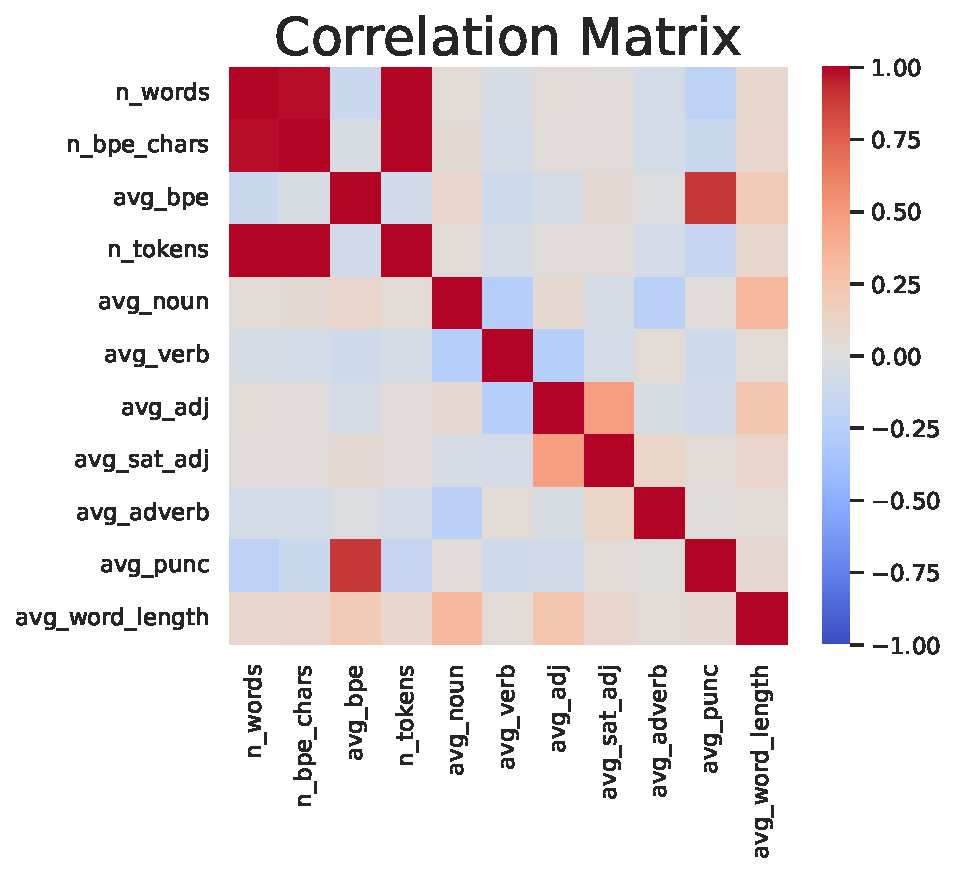
\includegraphics[width=0.75\textwidth]{figures/text_corr_matrix.pdf}
    \caption{Heatmap of the Pearson correlation matrix for the features in our machine translation feature engineering.}
    \label{fig:nlp_correlation_matrix}
\end{figure}

This heatmap provides a visual representation of the relationships between different features in our MT feature engineering process, allowing for a direct comparison with the original study's findings.



\subsection{Premodel}
\subsubsection{Image classification}
\subsubsection{Machine translation}


% at Timotej and Marko: this is the other option:
%\section{Methodology}
%
%    \subsection{Computer vision}
%        \subsubsection{Base model}
%        \subsubsection{Feature engineering}
%        \subsubsection{Premodel}
%    
%    \subsection{Natural language processing}
%        \subsubsection{Base model}
%        \subsubsection{Feature engineering}
%        \subsubsection{Premodel}



\section{Results}




\section{Discussion}
discussion

\subsection{What was easy}
answer

\subsection{What was difficult}
answer

\subsection{Communication with original authors}
answer
